\section{Process's perspective} \label{section:Process perspective}
\todo{Also reflect and describe what was the "DevOps" style of your work. For example, what did you do differently to previous development projects and how did it work?}

\subsection{Interactions and organization of developer team} 
The developer team stays in contact through a Microsoft Teams with regular meetings every Monday and usually one or two additional "stand up" type meetings throughout the week to check in on progress. Microsoft Teams is also used for links and resources as well as communication regarding individual tasks.

Major issues are typically done with everyone present, if they require important decisions, otherwise work is usually done individually or in groups of two or three people - depending on the complexity of the task ahead.

\subsection{CI/CD chain} 
For CI, we initially attempted to use TravisCI, as everyone in the group had encountered it. TravisCI was abandoned due to an overwhelming number of issues with files and folders not being added properly, in addition to secret handling being bothersome.

We instead settled for using GitHub Actions, which had all the features we wanted (triggers, stages, customizable images and non-local storage of secrets).

The following workflows are set up:
\begin{itemize}
    \item \textbf{Java CI with Maven}: Invoked on all pushes to the repository. It builds the Maven project using $mvn package$ and runs all tests, including integration tests on a remote test database. The workflow utilizes caching to ensure that Maven dependencies are not fetched on consecutive runs. 
    \item \textbf{Staging deployment}: Invoked on all pushes to the main branch. This workflow logs into DockerHub, builds and pushes the Minitwit docker image with database secrets. Afterwards it SSHs to the primary Minitwit server and fetches the Minitwit config files, including the docker-compose file. Immediately after all containers are torn down and rebuild using the newly pushed Minitwit image from DockerHub. Finally, a release is created with new commits linked and the backup server is redeployed similarly. In the downtime of the primary server the backup server obtains the floating IP and vice versa. 
    \item \textbf{Backup DB}: Once a day GitHub action SSH into the primary server and creates a database dump with time and date in the name. Created to minimize potential data loss.
    \item \textbf{Build LaTeX document}: When a push to develop occurs, the LaTeX files are fetched from the report folder and a pdf document is built. The LaTeX files are manually fetched from a remote Overleaf repository, as Overleaf facilitates the groups collaborative writing. 
    \item \textbf{SonarCloud}: Official SonarCloud GitHub action that builds and analyzes the Java project using \textit{mvn\_verify}. 
\end{itemize}
For secret handling we used Githubs Encrypted secrets. This ensured that no potentially harmful information was exposed in the GitHub Action workflows. Among secrets were DB connection strings, DigitalOcean access tokens, DockerHub credentials and SSH keys together with host information.


\subsection{Organization of repository}
The code is organized using a mono repository setup, having all code and scripts necessary to run the application gathered in a single repository. The team deemed this sufficient as everything located in the repository (apart from local dockerfiles and simulator) is involved in the deployment process and the code-base is small and simple enough that having multiple repositories would only increase complexity. 

\subsection{Applied branching strategy and development process} 
The main branch is used for the latest release, meaning that the code on this branch matches code found in production.

The develop branch facilitated the main development of the project and should always contain a working build. From develop each group member could create feature branches (\texttt{feature/logging} for example) and then merge back into develop once tested and approved. Develop could be subject to hotfixes, which would then be merged into main. The full process can be seen in \underline{\href{https://github.com/DevOps2021-gb/devops2021/blob/main/CONTRIBUTE.md}{CONTRIBUTE.md}}.

The group used GitHub issues to track development progress, labeling them as needed with tags such as \textit{bug}, \textit{documentation}, \textit{feature} and \textit{enhancement}. The status of each issue and the issues to focus on each week was tracked using GitHub's kanban board, having columns \textit{Todo}, \textit{This sprint}, \textit{In progress} and \textit{Done}.

\subsection{Monitoring} 
\label{subsection:monitoring}
Monitoring is set up using Prometheus and Grafana, where Prometheus is used to subtract data from the system, at the data is displayed on dashboards in Grafana.

The newest data points are collected and stored using \texttt{MaintenanceService.java}. Each data type is stored in Prometheus library's Gauge or Counter objects, which is registered with a unique name and help description. Data gathered is: the current CPU load, database information and response-time of each endpoint. The data is collected with an interval of 30 seconds. The configuration of Prometheus is found in \texttt{prometheus.yml}\footnote{\url{https://github.com/DevOps2021-gb/devops2021/blob/main/prometheus.yml}}.

On \textit{Grafana} are three dashboards:
\begin{itemize}
    \item \textbf{Minitwit DB info} shows information about the data stored in the database, e.g. the current number of users registered for the application \footnote{\url{http://144.126.244.138:3000/dashboard/db/minitwit-db-info?orgId=1}}.
    \begin{figure}[H]
        \centering
        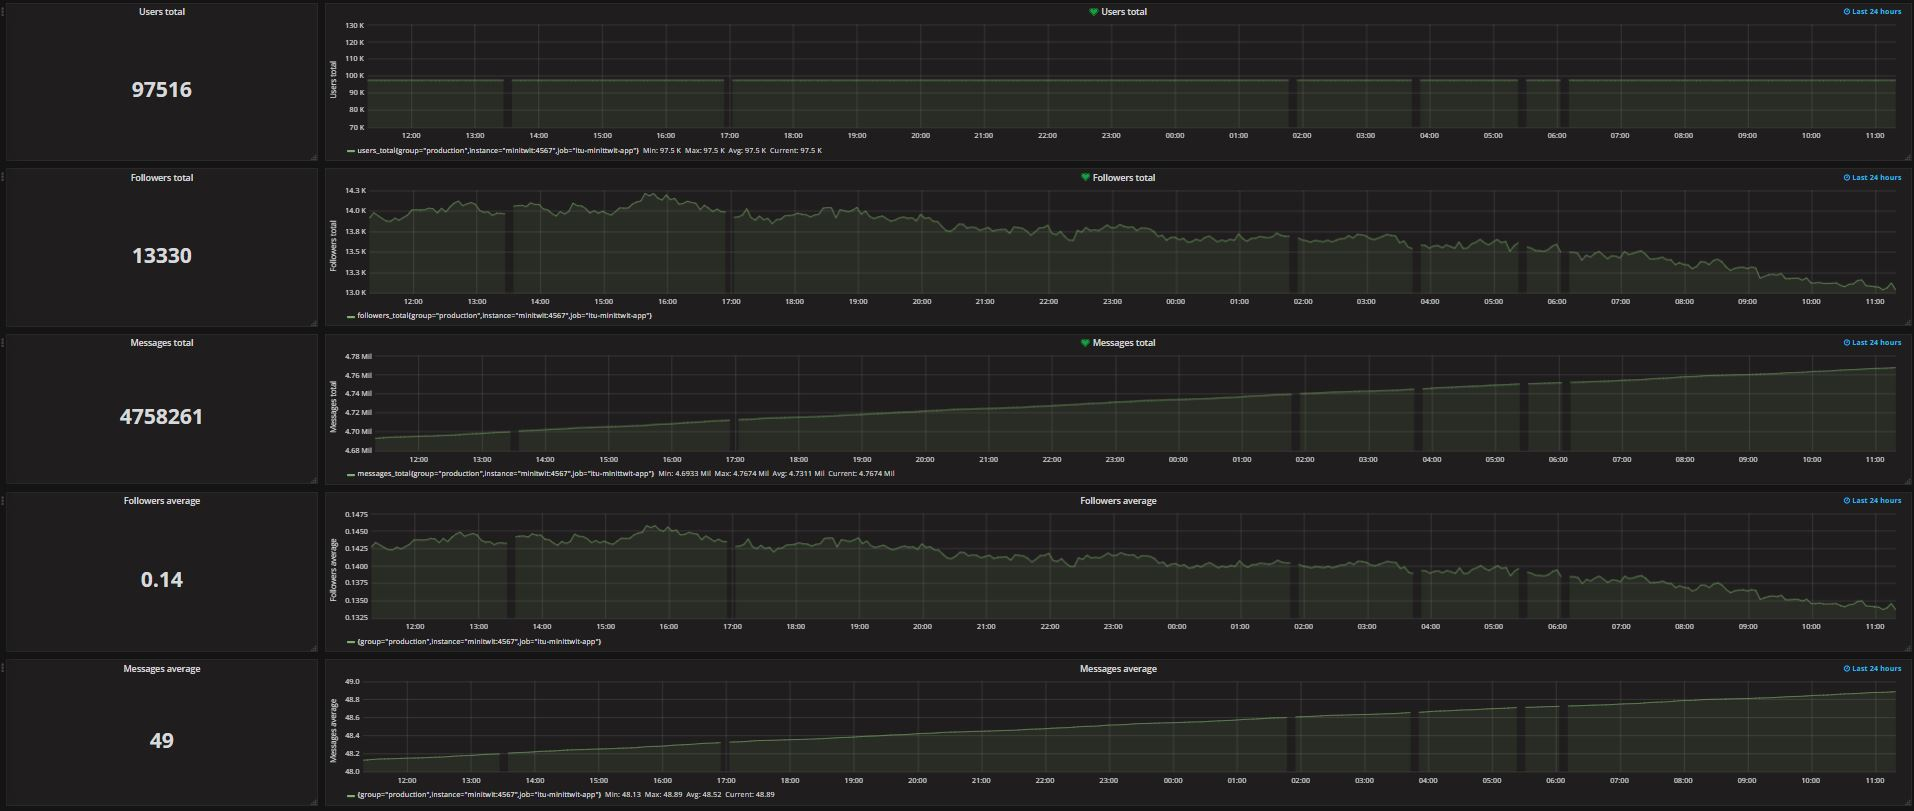
\includegraphics[width=1.0\textwidth]{images/Grafana_minitwit_db.JPG}
        \caption{Grafana dashboard minitwit db}
        \label{fig:grafana_db}
    \end{figure}
    
    \item \textbf{Minitwit request}\footnote{\url{http://144.126.244.138:3000/dashboard/db/minitwit-requests?orgId=1}} shows response times for requests to the system.
    \begin{figure}[H]
        \centering
        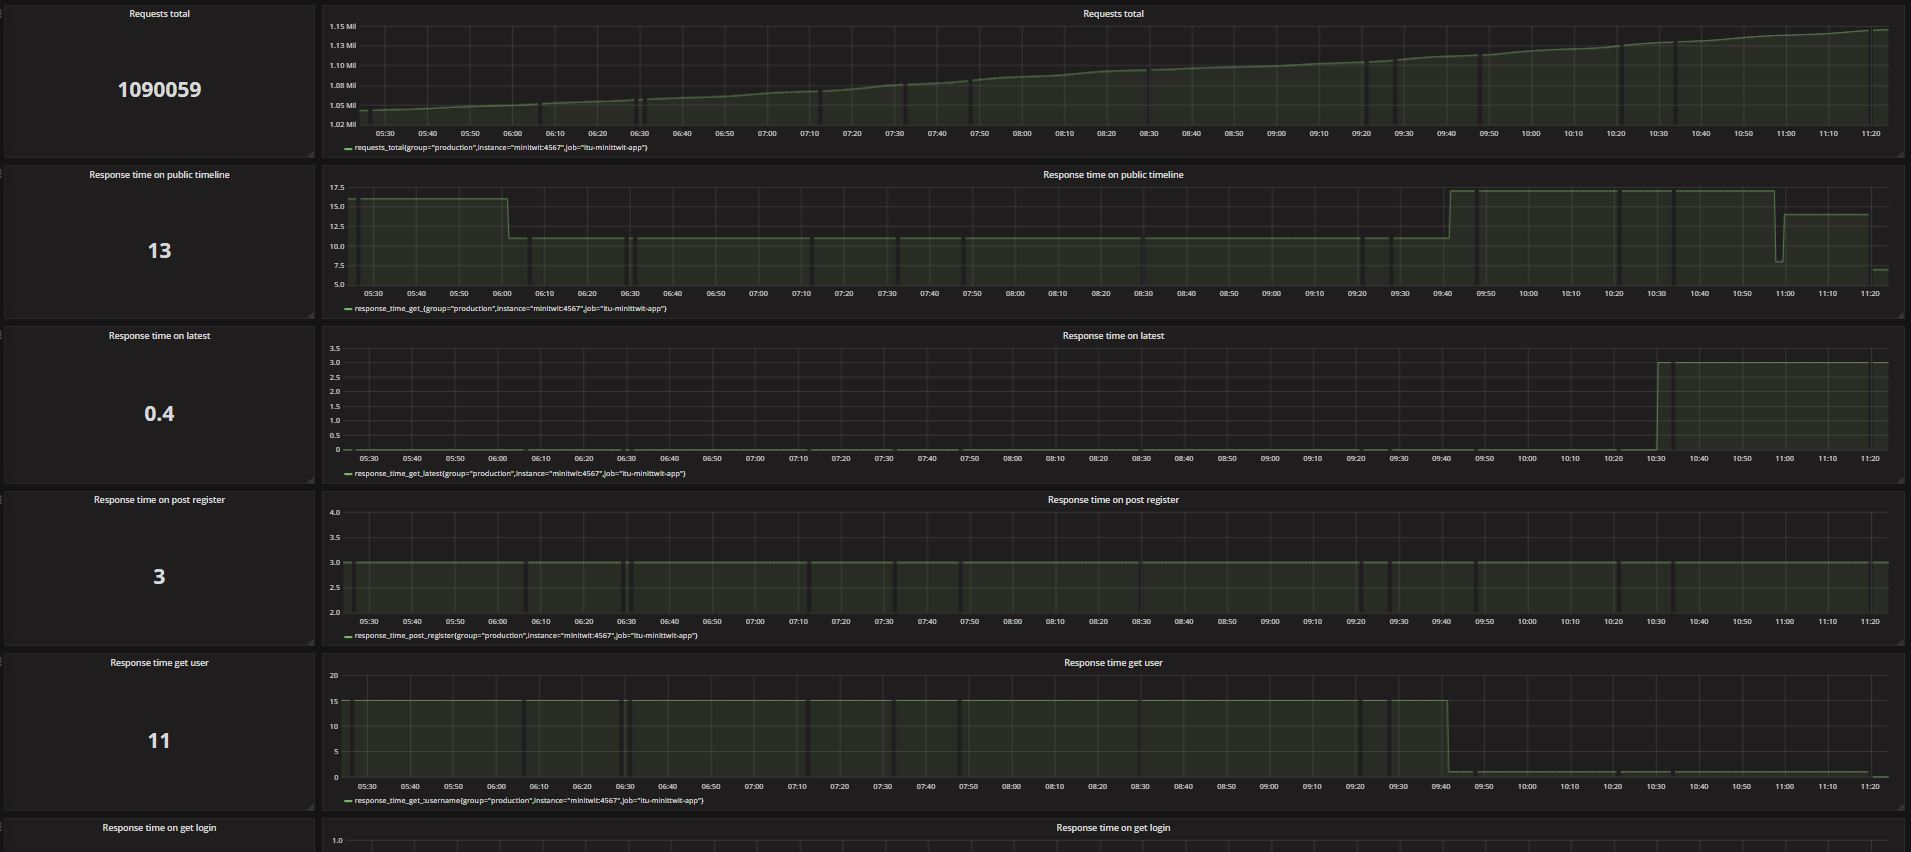
\includegraphics[width=1.0\textwidth]{images/Grafana_minitwit_requests.JPG}
        \caption{Grafana dashboard minitwit requests}
        \label{fig:grafana_requests}
    \end{figure}
    
    \item \textbf{Prometheus Stats}\footnote{\url{http://144.126.244.138:3000/dashboard/db/prometheus-stats?orgId=1}} shows the uptime of the system. The time is reset when the system is redeployed or if it goes down.
    \begin{figure}[H]
        \centering
        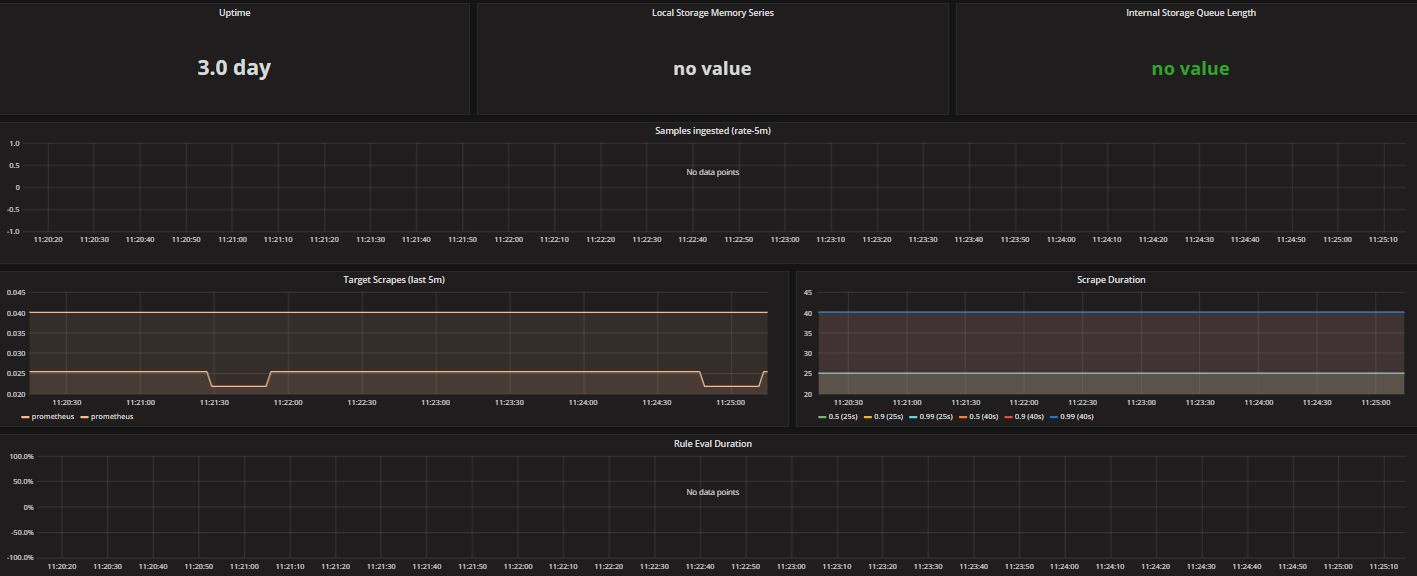
\includegraphics[width=1.0\textwidth]{images/Grafana_prometheous_stats.JPG}
        \caption{Grafana dashboard Prometheus Stats}
        \label{fig:grafana_prometheus}
    \end{figure}
\end{itemize}
The graphs in the dashboards show minimum, maximum and average of the plotted data. The graphs with a heart in the title contains alerts that every 60 seconds check if latest value is below a threshold, indicating that a critical error has occurred. When/if such an alert is triggered Grafana should be setup to email the members of the team, see section \ref{issues-maintenance}.

\subsection{Logging}
\label{subsection:logging}
Logging is set up as an EFK stack. Initially only exceptions were logged but during a test of the logging only one of three introduced bugs was detected, implying that the logging was insufficient. More detailed logging was introduced, now also logging requests and their payloads with the exception of passwords \todo{hashes eller rigtige?} which was removed. This change made all three kinds of bug show up in the log. The description of the experiment can be found in the wiki entry \underline{\href{https://github.com/DevOps2021-gb/devops2021/wiki/Catch-a-Bug-By-Looking-at-the-Logs}{Catch a Bug By Looking at the Logs}}.

Logging is done using Java's Logger object and through our helper-functions each print is extended with a classification/level. The print statements also get a code to easier filter actual warnings rather than messages containing the word 'warning'. The class printing is also added to the message for traceability

These measures allowed us to create filters for Grafana dashboards such that we could see all messages, all warnings and all of the different kinds of exceptions that could be thrown. 
\todo{log volumes, traces, exceptions}


\subsection{Security assessment}
In order to assess the security of the system two tasks were undertaken. A risk assessment was conducted and penetration testing was performed.

For risk assessment three assets to protect was identified: the web application, the database and the logging. The following potential threats were assessed:
\begin{itemize}
    \item Web application: SQL injection, cross site scripting, DOS, brute forcing login and insufficient logging and monitoring.
    \item Database: SQL injection through web application/API and lost authentication secrets.
    \item Logging: DOS attacks, brute forcing login page.
\end{itemize}

A risk analysis table was constructed and 11 scenarios and seven issues were identified and graded. For most of the scenarios actions had already been taken to prevent or mitigate the risks. For a few other scenarios possible actions were identified but not taken as they were not deemed necessary. The full details of the risks assessment can be found under \underline{\href{https://github.com/DevOps2021-gb/devops2021/wiki/Risk-assesment}{Risk Assessment}}.

For the penetration testing three tools were used: \textit{nmap}, \textit{Metasploit} and \textit{SQL map}. In each case no vulnerabilities were found. In addition to using \textit{SQL map} cross-site scripting was also tested manually in multiple browsers by trying to use script-tags in the message input field on the website. In all tested browsers the script tag was not rendered. Lastly, it was checked that traces of the tools run showed up in the logging. The full details of the penetration test can be seen in \underline{\href{https://github.com/DevOps2021-gb/devops2021/wiki/Penetration-testing}{Penetration testing}}.

Another group was supposed to perform a white hat attack on the system. Nothing was heard from the group and it must be assumed that they found nothing to report.% or tested another group by mistake.

\subsection{Scaling and load balancing}\label{subsection:scaling} 
The group first implemented the traditional Heartbeat with Floating IPs on DigitalOcean \footnote{\url{https://www.digitalocean.com/community/tutorials/how-to-create-a-high-availability-setup-with-heartbeat-and-floating-ips-on-ubuntu-16-04}}. Unfortunately this would only ensure that floating IP were switched to the backup and back when the entire machine would go down. We did not find a configuration of Heartbeat that would allow us to listen on a specific port, and switch floating IP's when the Minitwit service was down. We therefore decided to write two shell scripts to gain the sought after functionality. The first script\footnote{\url{https://github.com/DevOps2021-gb/devops2021/tree/main/heartbeat}} continuously runs on the secondary droplet checking the availability of the primary droplet, reassigning the floating-ip to itself should the application on the primary droplet go down. The second script would run on the primary droplet to reassign the floating IP to itself when it has restarted.